%% article.tex
%% V1.4b
%% 2015/08/26
%% by Michael Shell
%% see http://www.michaelshell.org/
%% for current contact information.
%%
%% This is a skeleton file demonstrating the use of IEEEtran.cls
%% (requires IEEEtran.cls version 1.8b or later) with an IEEE
%% journal paper.
%%
%% Support sites:
%% http://www.michaelshell.org/tex/ieeetran/
%% http://www.ctan.org/pkg/ieeetran
%% and
%% http://www.ieee.org/

%%*************************************************************************
%% Legal Notice:
%% This code is offered as-is without any warranty either expressed or
%% implied; without even the implied warranty of MERCHANTABILITY or
%% FITNESS FOR A PARTICULAR PURPOSE! 
%% User assumes all risk.
%% In no event shall the IEEE or any contributor to this code be liable for
%% any damages or losses, including, but not limited to, incidental,
%% consequential, or any other damages, resulting from the use or misuse
%% of any information contained here.
%%
%% All comments are the opinions of their respective authors and are not
%% necessarily endorsed by the IEEE.
%%
%% This work is distributed under the LaTeX Project Public License (LPPL)
%% ( http://www.latex-project.org/ ) version 1.3, and may be freely used,
%% distributed and modified. A copy of the LPPL, version 1.3, is included
%% in the base LaTeX documentation of all distributions of LaTeX released
%% 2003/12/01 or later.
%% Retain all contribution notices and credits.
%% ** Modified files should be clearly indicated as such, including  **
%% ** renaming them and changing author support contact information. **
%%*************************************************************************

\documentclass[journal]{IEEEtran}

\usepackage{cite}

\usepackage[pdftex]{graphicx}
\graphicspath{ {./images/} }
\usepackage{caption}

%\usepackage{amsmath}

\usepackage{algorithm}
\usepackage{algpseudocode}

%\usepackage{array}

%\usepackage[caption=false,font=normalsize,labelfont=sf,textfont=sf]{subfig}

%\usepackage{fixltx2e}

%\usepackage{stfloats}

%\usepackage{dblfloatfix}

%\usepackage{url}

\usepackage{hyperref}

% correct bad hyphenation here
\hyphenation{op-tical net-works semi-conduc-tor}

\algdef{SE}[SUBALG]{Indent}{EndIndent}{}{\algorithmicend\ }%
\algtext*{Indent}
\algtext*{EndIndent}

\newcommand{\LineComment}[1]{\State \texttt{/* #1 */}}


\begin{document}

\title{The Units of Permissionless Consensus: \\ Towards Mobile and Edge Computing}

\author{Eduardo Ribas Brito 
\\Supervisors: Ulrich Norbisrath, Eero Vainikko
\\Distributed Systems Seminar, Fall 2022
\\\emph{Institute of Computer Science}
\\\emph{University of Tartu, Estonia}
\\ eduardo.ribas.brito@ut.ee}

\maketitle

\begin{abstract}

This paper presents an overview of the consensus problem
applicable to permissionless environments. Starting from 
the classical roots of consensus in distributed systems,
transitioning to the more recent developments in the
field of permissionless consensus, this paper also reviews
the common approaches and architectural design of the most well known protocols, 
and discusses the trade-offs between the different strategies.
Finally, this paper points out the challenges that
permissionless consensus faces in the context of resource
constrained environments, such as mobile and edge computing.
It identifies and argues about the current approaches to address these challenges,
and shows potential research directions.

\end{abstract}

\begin{IEEEkeywords}
Consensus, Distributed Systems, Permissionless Consensus, Mobile and Edge Computing, Blockchain, Resource Constrained Environments.
\end{IEEEkeywords}

\section{Introduction}

\IEEEPARstart{L}{ong} has been the time when consensus started 
to be defined as a fundamental problem of distributed systems \cite{pease1980reaching, lamport2019byzantine, lamport1983weak}. 
Generally, consensus means reaching an agreement between multiple parties 
in the potential presence of faulty individuals. As per multi-agent systems, 
interacting over computer networks, consensus is thought to be the result 
of a coordination effort, such that those parties agree on some value at a 
given moment. Achieving consensus implies that the system shall be reliable 
and fault-tolerant. However, the consensus problem has been limited by some 
assumptions on the networks. The well-known "secure Byzantine-Fault-Tolerant 
multiparty consensus systems" that have been designed over the years are usually 
meant to work only with a set of known participants, faulty or not \cite{castro1999practical}. The 
other side of the coin is the permissionless consensus challenge, consisting of 
achieving agreement in an environment where the participants are unknown and 
untrusted \cite{nakamoto2008bitcoin, buterin2014next}. Plus, there are other intrinsic particularities of 
this type of networks, for example, their openness, and the lack of any kind of central 
authority. This adds another layer of complexity to the problem, as the participants 
are not only unknown and untrusted but can also join or leave the network at any time, 
freely choosing if they want to participate in the consensus protocol or not. Nevertheless, 
the problem of permissionless consensus can still be seen as a special case of the more 
general consensus and can still be formalized in the same way. In this paper, we will 
focus on consensus in permissionless systems, especially in the context of blockchain 
networks. We will reason about its meaningfulness, ultimately by trying to identify the units that 
may underpin consensus. We will also discuss the current state-of-the-art, with a 
particular interest in the shift of the consensus layer of these distributed networks 
to mobile and edge computing environments, for which computationally expensive consensus 
algorithms are impractical and unfair.

\section{Related Work}

\subsection{Classical Consensus}

The establishment of a definition for the problem of reaching agreement in a distributed 
system was pioneered by Lamport et al. in \cite{pease1980reaching}. 
The authors defined consensus as the problem of agreeing on a single value among a set of processes, 
in the presence of faulty entities. The first consensus algorithms were designed for 
synchronous systems, where the communication between the processes is reliable, and the 
delay is bounded. However, these initial attempts failed to cover the different types of 
faulty behavior. Along with the establishment of the famous Byzantine Generals Problem, 
the first solutions, not only for dealing with treason, but also for unreliable communication 
channels, or any other kind of arbitrary Byzantine behavior, were 
also proposed by Lamport in \cite{lamport2019byzantine,lamport1983weak}. The solution was a synchronous 
mechanism that used a set of leaders to reach consensus. Multiple practical implementations 
and optimizations to this solution have been proposed in the literature. 

\subsection{Asynchronous Byzantine Consensus}

The first practical asynchronous consensus algorithm was later proposed by Castro and Liskov in \cite{castro1999practical}. 
And naturally, after that work, many other asynchronous consensus algorithms have appeared. 
However, all of them are based on the assumption that the number of faulty processes is less than 
a certain threshold. Additionally, the assumption of a known set of participants is also made, as well as their roles 
in the consensus protocol. These are very strong assumptions that limit the challenges that can be addressed, 
for example, the impossibility to know the participants beforehand as they may participate anonymously, or dynamically.

\subsection{Permissionless Consensus}

The advancements of the internet 
more than potentiated the revolution and what we now call the permissionless consensus problem was 
finally born. Without forgetting the previous attempts, the first practical permissionless consensus algorithm was 
proposed by Nakamoto in \cite{nakamoto2008bitcoin}. It is a proof-of-work consensus protocol that resembles a "replicated 
state machine" where the independent participants reach agreement not only about transactional values, 
but also about their order - naturally forming the underlying structure of what is now known as a blockchain. 
"Proof-of-work is essentially one-CPU-one-vote" and this is the novelty 
introduced by Bitcoin \cite{pass2016hybrid,pass2016hybrid2}. The focus shifted 
for decentralized systems and after proof-of-work many other consensus mechanisms have been proposed, 
based on different consensus units, like proof-of-stake, proof-of-space, proof-of-authority, etc. The chaotic 
diversity of new consensus protocols gave also room for endless reviews, overviews and comparisons \cite{survey-dist-consensus, BAMAKAN2020113385, 8400278, natoli2019deconstructing, 8629877, 9376868, BOURAGA2021114384}. 
The authors of these surveys often put multiple dimensions into comparison, like fault tolerance, scalability, or energy consumption,
and, among those, some focused their efforts on mechanisms that may work in resource-constrained networks \cite{9104713, 8168250, queralta2021blockchain, SALIMITARI2020100212}. 
This paper will try to identify the common conclusions from these comparisons, while looking into the state-of-the-art and novel approaches for running permissionless
consensus protocols in mobile and edge devices.

\section{The need for permissionless consensus}

\subsection{Permissioned vs Permissionless}

Following the line of the previous sections, it has been reasoned about the need 
for permissionless consensus when there are already well known and established consensus protocols
that work in trusted environments \cite{castro1999practical, miller2016honey}. However, even those protocols have
their own limitations, not only in terms of trust, fault-tolerance, centrality, permissions,
or bottlenecks, but also in terms of scalability \cite{miller2016honey}. Trying to put some effort on decentralization, 
Byzantine-Fault-Tolerant consensus protocols are not known for their performance when the network grows
in size. The more participants there are, the more messages need to be exchanged
between them, and the more time it takes to reach consensus, even if assuring deterministic finality \cite{decker2016bitcoin}. 
This is a problem that is not only related to the number of participants, but also to the
communication fashion and bandwidth, and the computational capacity of the devices that
participate in the consensus protocol. 
Summing up, the need for permissionless consensus is then justified by the fact that
permissioned protocols are not compatible with the requirements of the new generation of
distributed systems, especially in the context of blockchain networks. 
These requirements include dealing with today's sparse networks of anonymously and dynamically
participating devices, without interrupting consensus and while battling Sybil attacks \cite{8629877, survey-dist-consensus}.
Fundamentally, the permissionless consensus problem is the need for a consensus protocol that
can be run in a distributed and decentralized environment, where the participants are unknown and untrusted,
and where the network is bigger, sparser and unpredictably less reliable.

\subsection{Allowances and goals}

Technically, permissionless environments allow for larger networks
that depict lower connectivity between the participants. Operationally,
everything is expected to happen in an asynchronous or partially synchronous fashion, 
and the number of transactions is expected to be smaller than the 
permissioned counterparts. Nevertheless, participation is free, and the
governance is not centralized, but rather distributed and public. 
The identity of the participants is secured or semi-secure as it often relies on
pseudonymity for protecting the nodes' identity, while enabling full transparency 
in regard to the rest of the network's content and operation \cite{xiao2019distributed}.
The goal of permissionless consensus, as generally for any consensus protocol, is to reach
agreement on a single value, or a set of values. However, due to the nature of the
protocols, the values that are agreed upon end up establishing the serialization of the
transactions that are executed in the network, and so establishing time consciousness and 
total order of the events \cite{8629877}.

As pointed out by \cite{xiao2019distributed, 8629877} and then referenced by \cite{survey-dist-consensus}, 
similarly to the permissioned counterparts, permissionless consensus protocols 
aim at achieving the following properties: Termination, Agreement, Validity, 
and Integrity. Without going into a lot of details, of these properties, 
Agreement and Integrity are the most important ones, as they are the ones that
guarantee the correctness of the consensus protocols. Termination and Validity
are generally related to any classical consensus problem.

\begin{figure}[h]
  \centering
  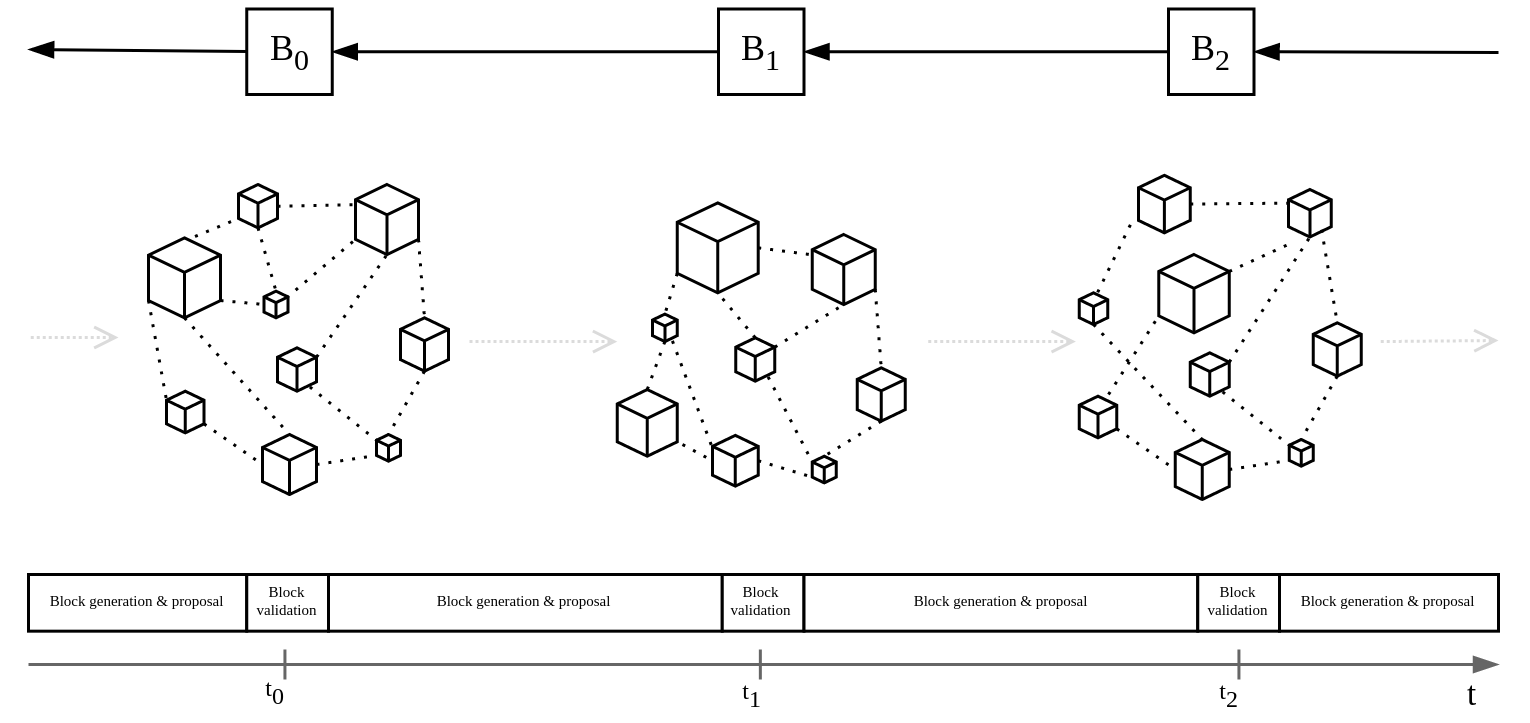
\includegraphics[width=\columnwidth]{building-blocks-consensus.png}
  \caption{An illustration of the permissionless consensus building blocks - 
  the block generation and proposal phases followed by the block validation, 
  along with frequent network topology changes and the consequent serialization of the information.}
  \label{fig:building-blocks-consensus}
\end{figure}

\subsection{The building blocks of permissionless consensus}

Also described in \cite{survey-dist-consensus}, very concisely, the 
way to achieve an operating protocol, as seen in the mainstream blockchain
networks, is by first generating the agreeable value, 
in this particular case, a block and its proof, disseminating the information 
to the rest of the network, followed by the eventual validation and 
acceptance of the block by the rest of the nodes. This is the moment when consensus is reached (See Fig. \ref{fig:building-blocks-consensus}).
Nevertheless, during the whole process, a fair and somewhat predictable incentive mechanism 
is also needed, that rewards the participants for their honest effort in reaching consensus, and
punishes the ones that are not behaving correctly. These incentives are of major importance
in this very context of permissionless consensus. 
These building blocks form the basis of the inner functioning of Bitcoin itself \cite{nakamoto2008bitcoin},
and are replicated with some variations in the other permissionless networks \cite{buterin2014next}.
For example, there are some networks that do not have a proof-of-work mechanism,
but rather a proof-of-stake, or a proof-of-space, or a proof-of-authority mechanism, etc.
when it comes to the generation of the block and its existential and later verifiable proof.
All the other pillars are generally the same \cite{survey-dist-consensus}.
The next sections will try to give a more detailed overview of these 
block generation proof units.

\section{Proof-of-Work as a reference}

\subsection{The block generation}
  
In the classical Nakamoto consensus protocol, the generation of a block, to be proposed
for further network agreement, complies with the unit of computational work needed to
create, or rather find, a verifiable proof of the effort spent on assembling the block \cite{nakamoto2008bitcoin}. 
This essentially requires brute forcing the search for a cryptographic hash value for the
aggregation of the block information with a nonce, such that this hash value satisfies
a difficulty threshold (See Algorithm \ref{alg:BlockGeneration}), which gets adjusted dynamically over time, to maintain the network overall 
requirement for the block generation interval \cite{8629877, survey-dist-consensus}.

There are a couple of particularities that need to be mentioned. First, the block generation
is of probabilistic nature, as the nonce is a random value, and the hash function is a one-way function.
Allied to this, increasing the hashing power is not an easy task, which consequently allows for tackling Sybil attacks,
despite the permissionless and pseudonymity nature of the network. Plus, the incentive mechanism
also plays a role in this regard, by naturally incentivizing honest participation.
The block generation interval, forged by the adjustment of the difficulty
threshold, is also of major importance because it reduces the fork probability and
allows for the timely propagation of proposed blocks, guaranteeing consensus
in the presence of an honest majority of the hashing power \cite{garay2015bitcoin, natoli2019deconstructing}.
This probabilistic finality shifts the 1/3 BFT threshold to a 1/2 threshold.

\begin{algorithm}
  \caption[short]{BlockGeneration}\label{alg:BlockGeneration}
  \begin{algorithmic}[1]
    \Function {}{}
      \State $Block Header \gets Transaction \ Merkle \ Tree \ Root$
      \Indent
        \State $| \ Hash \ of \ the \ last \ Block$
        \State $| \ Timestamp$
        \State $| \ Other$
      \EndIndent
      
      \LineComment{the preceding zero bits in $target$ depict the mining difficulty}
      \While{$Hash(BlockHeader \ | \ nonce) \geq target$}
      \State Increment $nonce$
      \EndWhile
      \State \Return new block
    \EndFunction
  \end{algorithmic}
\end{algorithm}

\subsection{Trade-offs and trilemma}

Despite the harmony of all the aforementioned clever characteristics,
the proof-of-work mechanism has some well known drawbacks. 
First, the block generation is computationally expensive, and so, the
energy consumption associated with it is also high. This is caused by the
dynamically adjusted difficulty threshold, which is a function of the block 
generation interval. For example, in the Bitcoin network, to maintain the 10 
minutes interval, the hashing difficulty
increases with the increase of the hashing power, and so too the energy needed for computing that proof. 
However, reducing the block generation interval would increase the
probability of forks, which results in a more frequent waste of useful work,
loosening the security of the network. Increasing the block size would also
have the same security effect due to the increased propagation delay \cite{8629877, natoli2019deconstructing}.

As pointed in the literature, the design of these consensus mechanisms
shall aim for a protocolar choice between a set of properties that form a trilemma (See Fig. \ref{fig:trilemma}): 
Security, Scalability, and Decentralization.
Summarizing, relaxing the security requirements may allow for more scalability, both of which,
consequently, have hands tied with decentralization. These trade-offs are of practical
consideration when defining the network goals and use cases \cite{survey-dist-consensus}.

\begin{figure}[h]
  \centering
  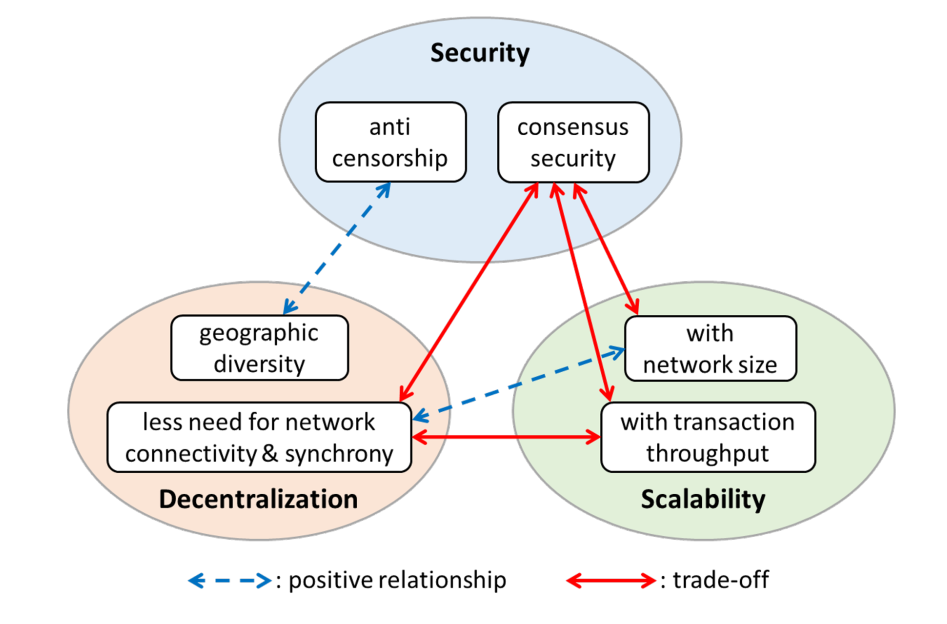
\includegraphics[width=\columnwidth]{trilemma}
  \caption{From \cite{survey-dist-consensus}, the blockchain consensus trilemma and its inner relations.}
  \label{fig:trilemma}
\end{figure}

\section{Alternatives to Proof-of-Work}

\subsection{Proof-of-Stake based protocols}

At this point, we can exercise the imagination and extrapolate the
previous block generation mechanism to a \emph{Proof-of-Something} 
pseudo-random competition in which an entity in possession of a higher
amount of a certain resource, either computational power, or stake, 
or certain currency, or a higher amount of storage space, etc., guarantees
a higher probability of leading the block generation and proposal, and
consequently winning the acceptance by the majority. This is the essence of
the Proof-of-Stake consensus protocol, as a derivative of the Proof-of-Work
mechanism, where a stake is a traceable and verifiable amount of a certain
unit, token or currency, that is owned by a certain entity that wishes to
participate in the consensus protocol. The stake works as a form of collateral
that is used to guarantee the honesty of the entities, in an attempt to
reduce the Sybil attack probability. And, generally as in Proof-of-Work, 
the higher the stake, the higher the probability of leading the block generation 
and proposal. Proof-of-Stake is, indeed, a more energy efficient consensus protocol,
however, this adds up to nothing, especially when compared to the already proved
BFT solutions, if centralization is a functional requirement, 
or unfair advantage is a potential trait. 
These limitations, along with other security concerns, may push away the 
participation of resourceless entities, and consequently, affect the network
decentralization and security.

\subsubsection{Chain-based and Committee-based protocols}

Due to the self-contained nature of this type of protocols, where the
attestation of the stake is done inside the network, multiple classes
of Proof-of-Stake can be distinguished by the way the meaningfulness of
the stake is defined and employed. For example, there are the simplest forms of \emph{PoS} that inherit most
of the characteristics of the Proof-of-Work mechanism, but with the
stake as part of the block generation and hashing proof (See Algorithm \ref{alg:PoSBlockGeneration}).
These are commonly referred to as Chain-based \emph{PoS}, inheriting also the
fault-tolerance properties of the Nakamoto consensus protocol.
Committee-based \emph{PoS} protocols, on the other hand, are more complex,
and based on the idea of a committee of entities that are 
selected to lead the block generation and proposal. The committee is
formed by a subset of the network entities, and the selection is done
based on their stake. Usually, the selection takes the form of a random
sequence of stakeholders, where the probability of being selected
for every spot is proportional to the stake. That sequence is then 
consciously timed to orderly pace the block generation and proposal, 
by the current slot leader. Examples of this type of mechanisms are
the \emph{Ouroboros} \cite{kiayias2017ouroboros}, \emph{Ouroboros Praos} \cite{david2018ouroboros} protocols
or \emph{Snow White} \cite{daian2019snow}. The longest chain rule is
still applied, with probabilistic finality, and the 1/2 threshold is
still required or tolerated for the network to reach consensus. Nonetheless,
Committee-based \emph{PoS} protocols may not pair well with decentralization and 
increase in the committee size, which deteriorates the performance of the
protocol. Several improvements have been proposed to tackle not only this
issue, but also the security of the committees which, smaller, could be more
vulnerable to targeted attacks \cite{david2018ouroboros}.
  
\subsubsection{BFT-based protocols}

These aim at achieving deterministic finality, by employing a BFT
consensus protocol, not at the block proposal level, but at the
block acceptance level. The idea is to have a free flow of blocks
proposed by the network, but to have a quorum of entities that
are responsible for the block acceptance. The block generation and proposal mechanism
can be of any kind, for example, Chain-based \emph{PoS}, or Committee-based \emph{PoS},
or even pure Proof-of-Work. The block acceptance layer then allows
for a deterministic acceptance of the blocks, by having a sort of permissioned
BFT consensus protocol, with the trivial 1/3 Byzantine tolerance. The most well known examples
and variations are the Tendermint \cite{buchman2016tendermint} and the new Ethereum Casper 
\cite{buterin2017casper} protocols.

Delegated Proof-of-Stake (DPoS) is a variation of the BFT-based protocols,
where the consensus group is formed by a subset of the network entities,
which are selected by the network, with a voting mechanism based on the
delegation of stake. The consensus is then achieved using a typical 
PBFT protocol, with the usual 1/3 Byzantine tolerance.

\begin{algorithm}
  \caption[short]{PoSBlockGeneration}\label{alg:PoSBlockGeneration}
  \begin{algorithmic}[1]
    \Function {}{}
      \State $Block Header \gets Transaction \ Merkle \ Tree \ Root$
      \Indent
        \State $| \ Hash \ of \ the \ last \ Block$
        \State $| \ Timestamp$
        \State $| \ Other$
      \EndIndent
      
      \LineComment{the preceding zero bits in $target$ depict the mining difficulty}
      \While{$Hash(BlockHeader \ | \ clockTime) \geq target \times stake $}
      \State Increment $clockTime$ by a constant $tickInterval$
      \EndWhile
      \State \Return new block
    \EndFunction
  \end{algorithmic}
\end{algorithm}

\begin{figure*}[h]
  \centering
  \captionsetup{justification=centering}
  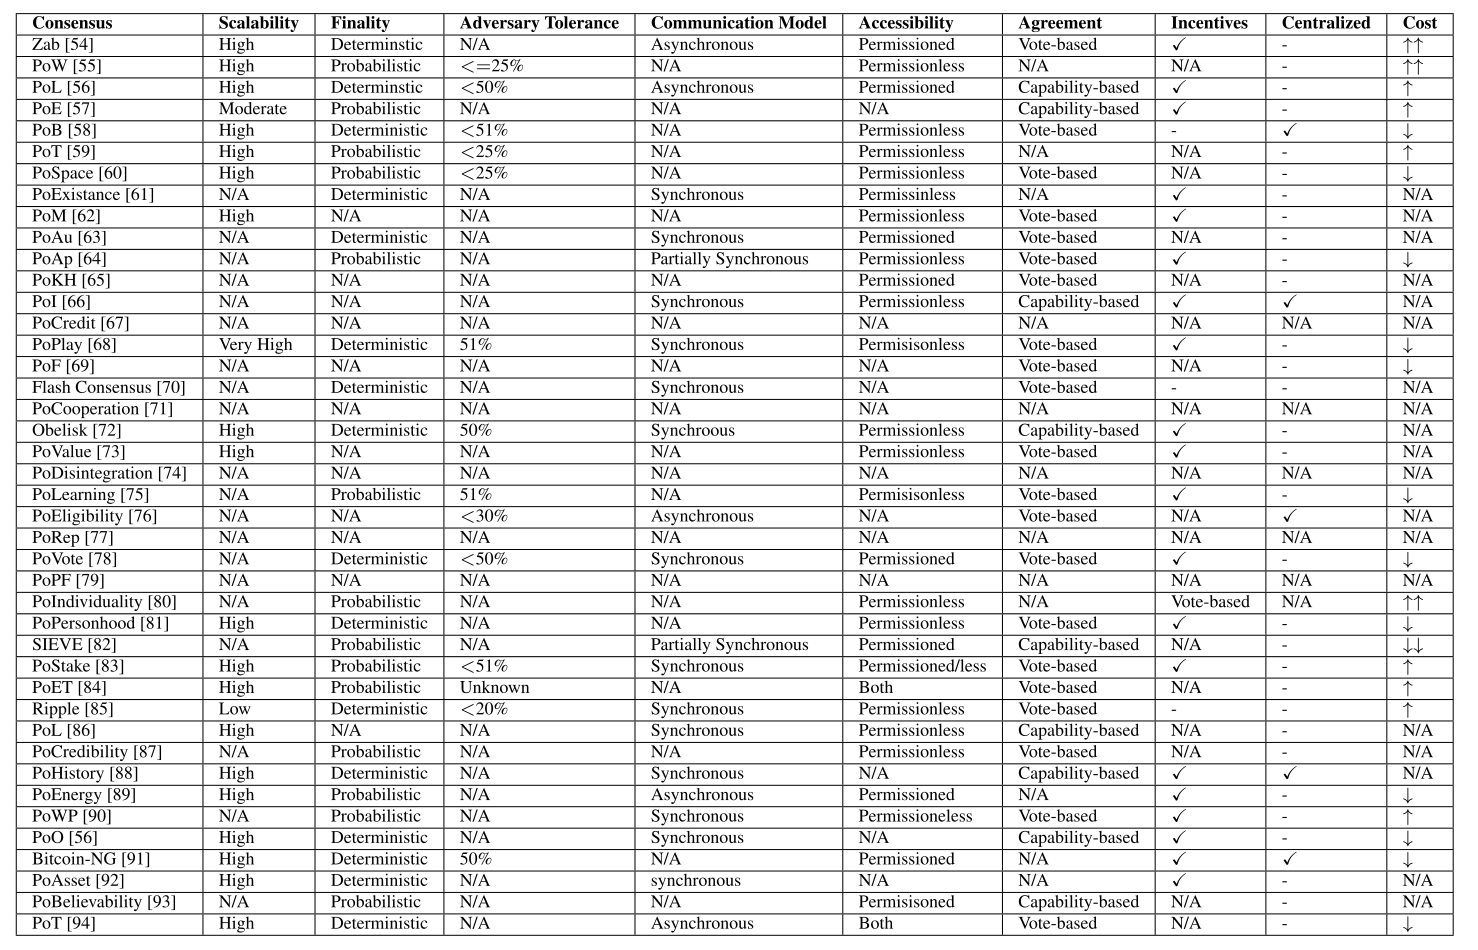
\includegraphics[width=\textwidth]{proof-alternative-consensus}
  \caption{From \cite{9376868}, an extensive list of pure proof alternative consensus mechanisms.}
  \label{fig:proof-alternative-consensus}
\end{figure*}

\subsection{Proof-of-Something Else}

Idealized and inspired by Proof-of-Stake, extending or adapting Proof-of-Work
became a popular trend in the blockchain community. The main idea is to
replace the computational power with some other resource, that is
more scarce, or more valuable, or more verifiable, or more traceable, etc.,
or to combine multiple resources, or even to add extra requirements to 
pure Proof-of-Work. From Proof-of-Meaningful-Work, or Proof-of-Luck, 
to Proof-of-Work-Time, going through Proof-of-Humanity, or Proof-of-Personhood, there
are countless and exotic variations of these mechanisms, and the list is growing \cite{token-economy-gitbook, 9376868}.
Not that every one of them has a big potential for entirely solving the permissionless consensus problem,
but each one of them may tackle different use cases where consensus needs to be reached, 
and where different resources are available to make the agreement happen \cite{BOURAGA2021114384, 9376868}.

\subsubsection{Proof-of-Space} established itself as a popular alternative among those.
The goal is to replace computational power with storage space,
and if possible give it a meaningful usage. Proof-of-Retrievability is
a cited example of this type of protocols, where the storage space is
used to store a large amount of relevant or public data, and the retrieval of that data
is used as a proof of the storage usage \cite{juels2007pors}. Despite the reciclability 
of the storage space, as a resource that could be a good alternative
to computational power, this algorithm has its own fatal flaws, depending
mostly on a central dealer for randomness as well as for consensus fairness.
Other reported Proof-of-Space variants may not even attempt to store/retrieve any meaningful data.

\subsubsection{Proof-of-Authority} is another well known derivative
which, in effect, is a form of Proof-of-Stake, where the stake is the 
identity of the entity, that has been verified, scrutinized and
approved by the network, giving it the right to participate in the
closed consensus group. The consensus protocol, if not a BFT protocol, 
can follow the style of a Proof-of-Work protocol, depending on the 
requirements of the network - a choice that may shape the fault tolerance,
decentralization, security and performance of the network \cite{survey-dist-consensus}.

\subsubsection{Proof-of-Elapsed-Time} is another alternative to \emph{PoW},
especially targeting the intensive mining issue, that has been proposed 
by Intel. The idea is to simulate the mining process by using a
randomized time delay, which is proportional to the amount of work
that would be required to mine the block. The time delay is then used to pace the
block generation and proposal, and the block acceptance can be performed
using a BFT protocol \cite{olson2018sawtooth}. This solution, however,
is not a viable alternative to other, permissioned and permissionless, approaches, 
by holding strong and centralized hardware requirements, 
as the computations require a trusted execution environment
(TEE) to establish the trust among the participants. Some efforts have been made
to combine the TEE feature with Proof-of-Stake, in order to achieve a
more decentralized and secure protocol, but the 
same hardware requirements are still a major issue.

\subsubsection{Proof-of-Location} may be an alternative for envisioning a future where
consensus is achieved by taking advantage of the dynamism and easiness of movement, placement and 
tracking of smaller and more location-versatile devices, such as mobile phones, IoT devices, etc.
The idea behind this approach is to use the location and movement of these devices 
as a proof for the consensus. It relies on the location validation by close proximity, 
for example, using low-range communication channels, either by proving the location
of the device at a certain point in time, or by proving their proximity to other devices.
Incentive mechanisms may play an important role to prevent location spoofing, collusion, etc. \cite{natoli2019deconstructing}.
These protocols are getting increased attention, especially in the context of IoT, 
with the provision of decentralized, permissionless and autonomous networks of 
low-powered devices that can be used for providing location verification services \cite{9376868}.

\subsection{Other approaches}

\subsubsection{The XRP Ledger Consensus Protocol} powers the XRP Ledger in a
low-latency, high throughput, and  BFT fashion. The network itself operates somewhat
differently from the other blockchain references, and treats transactions as atomic units of 
the ledger. These transactions are collected by the nodes and relayed to the
nodes' UNL (Unique Node List), which is a list of peers that are trusted by that current
entity. At every epoch, multiple rounds are needed to filter transactions and vote 
on the next state of the ledger. This voting happens at the 
UNLs' level, which are expected to be overlapped by a certain percentage,
in order to achieve the artificial vote threshold for globally accepting the transactions.
That threshold defines the fault tolerance of the protocol, and is set to 80\%, which 
bounds this protocol to a 1/5 BFT allowance \cite{schwartz2014ripple, chase2018analysis}. 
Despite that limitation, when compared to other BFT protocols, this protocol seeks to trade 
fault tolerance for performance, by having lower connectivity and less message exchanges. 
However, it is still expected high synchrony within the UNLs. Given these characteristics, this protocol
may be more suitable for permissioned networks, and, in terms of network size,
is seen as not as scalable and decentralized as the permissionless ones \cite{survey-dist-consensus}.

\subsubsection{DAG structures} may diverge from the previous approaches with an envisioned 
non-linear structure for the result of the consensus attestations. The choice resides in 
directed acyclic graphs that should expand and physically connect, further in time, the new
data appended to the network. The data, which is typically held in the vertices of the graph, 
can have more or less granularity, either by storing blocks of transactions, or raw transactions directly.
This design decision may pose new potential challenges, related to the verification and finalization of
the consensus protocol. Currently, those two approaches are then distinguished as \emph{blockDAG} and 
\emph{txDAG} \cite{survey-dist-consensus}. 
The block-based DAG approach diverges from the traditional blockchain structure by flexibly 
connecting every new block to multiple previous blocks. The rest of the protocol may work in the same way 
as the traditional Proof-of-Work, however, this new feature yields new security considerations. These protocols
are theoretically designed for very high throughput in permissionless environments, but the security trade-offs
are still not well-known \cite{sompolinsky2018phantom}.
In a transaction-based DAG, every vertex holds one transaction, that is connected to previous vertices. 
All the sibling vertices shall then represent disjoint transactions to successfully deal with history and conflict
resolutions. Two well-known examples of this approach are IOTA Tangle \cite{popov2018tangle} 
and Nano \cite{lemahieu2018nano}.
The former is of particular interest, as it is especially designed for IoT applications, low-powered devices, and
microtransactions. The protocol states that every new vertex needs to be connected to two previous vertices, 
therefore approving the parent transactions, as an incentive mechanism for honest behavior \cite{survey-dist-consensus}. 
The users are the ones to submit transactions, generating and attaching a \emph{PoW} proof to it and 
so guaranteeing probabilistic finality with 1/2 fault tolerance. This solution may indeed pair well with 
decentralization and scalability, however, there are known security issues related to the
easiness of growing malicious parallel branches with little computational effort, and those issues have been 
addressed by the introduction of an undesirable centralized solution. 
Other interesting and worth mentioning protocols are the ones that combine the DAG structure with the BFT consensus, 
such as the Snowflake-Avalanche protocol \cite{rocket2018snowflake}.

\section{Resource-Constrained Networks}

\subsection{Characteristics}

Resource-constrained networks are a class of networks that are characterized by the
limited access to resources, such as energy, bandwidth, storage, etc.
These networks are typically seen in IoT applications, where the devices are
usually low-powered, with limited computational resources, but are expected to 
collectively operate with high availability, at least the network as a whole, 
preferably without the need for frequent maintenance.
These networks are also expected to be dynamic, with frequent changes in the network
topology, by the unpredictable addition and removal of nodes. 
The nodes are also expected to be heterogeneous, with different capabilities, and may be
connected to the network through different communication channels. 
Mobility may also be a feature, as the nodes may spatially move around, 
and may directly pair with different nodes at different moments.
The nodes may also be individually unreliable, untrusted, uncoordinated, unmanageable, may fail at any time, 
and may be disconnected from the rest of the network.

Nowadays, the typical resource-constrained networks follow a centralized architecture
with a client-server model, where the network is controlled by a single entity,
which is responsible for the management of the nodes, including authentication,
authorization, and communication. This single-point-of-failure is also a major
scalability bottleneck, and a maintenance burden, as the network grows in number of devices \cite{SALIMITARI2020100212}.

\subsection{Challenges}

Having in mind these characteristics of resource-constrained networks,
and the drawbacks of the centralized architecture, it may be postulated the 
need for a decentralized or permissionless shift that addresses some the most important challenges
of these deployments \cite{SALIMITARI2020100212}:

\begin{itemize}
  \item \emph{Scalability}:  in terms of the number of available devices - decentralizing may allow
  for better, faster and less costly maintenance of the network, assuring more availability and reliability
  and cutting the single-entity dependency;
  \item \emph{Security}: in terms of the network as a whole - removing the single-point-of-failure 
  may reduce the attack surface, and may also allow for more flexible and dynamic security policies;
  \item \emph{Privacy}: in terms of the network data exchange features - decentralizing may allow for
  a user-centric approach, where the users are in control of the data that is shared with the network; 
\end{itemize}

Permissionless consensus is a promising solution for these challenges, as an enabler for
decentralized environments. The use cases for these networks are diverse. Nevertheless,
as long as consensus is achieved, the network as a whole can be abstractly seen and used
as a trusted entity that runs as a trustless decentralized service. Applications may then
be built on top of it, and the network may be used as a platform for other services \cite{queralta2021blockchain}.
However, there are some key aspects that need to be addressed
in order to make this approach viable for resource-constrained networks, as we saw in the previous section:

\begin{itemize}
  \item \emph{Resource consumption}: the consensus protocols should be resource-efficient, for example, in terms of energy, bandwidth, or storage, 
  as the nodes are expected to be low-powered devices, with limited computational, communication, and storage resources;
  \item \emph{Heterogeneity}: the consensus protocols should account for different device characteristics, 
  as the nodes are expected to be heterogeneous in terms of their capabilities;
  \item \emph{Fault tolerance}: the consensus protocols should be fault-tolerant, as the nodes are expected to be unreliable, 
  untrusted, uncoordinated, or unmanageable;
  \item \emph{Openness}: the consensus protocols should be open and trustless, as the nodes are expected to be 
  dynamically added and removed from the network;
  \item \emph{Security}: the consensus protocols should be resistant to a multitude of new attacks,
   especially if it turns out to be easy for malicious entities to overcome resource constraints;
\end{itemize}

The overall theoretical properties of the consensus protocols still need to be taken into account,
as the goal is to have a proved functional mechanism that achieves Termination, Agreement, Validity, and Integrity,
while playing with the trade-offs imposed by the trilemma (See Fig. \ref{fig:trilemma}) \cite{survey-dist-consensus}.

\subsection{Related Work}

There have been several attempts to address the challenges of resource-constrained networks,
and to understand the limitations of the existing consensus protocols in this context.
A common conclusion is that the existing protocols are not suitable for these networks,
due either to the high resource consumption, or to the centralization of various aspects of the protocol,
or also to high communication overheads, that are translated to high latency and low throughput \cite{SALIMITARI2020100212},
making these protocols unsuitable for resource-constrained applications. Other concerns are
the high space consumption, to store the older blockchain information, or the security issues, 
as some attempts to overcome the resource constraints may lead to new vulnerabilities,
which may be exploited by malicious and more powerful entities.

A thoroughly mentioned approach is the IOTA Tangle protocol \cite{popov2018tangle}, which
presents a friendly design for resource-constrained networks, infinitely scalable, and with low latency.
However, there are still known security and centralization limitations, as presented in the sections before \cite{8168250}.
Another concept that has been explored is sharding \cite{SALIMITARI2020100212, queralta2021blockchain}, which is a
technique that allows for the partitioning of the network into smaller subnetworks,
that are then managed by different entities, validating transactions in parallel. 
This approach may be used to overcome the scalability bottleneck,
but it may also introduce new issues that are still to be researched.
Frankly, there are indeed some well established protocols that, all in all, can be adapted to networks with
resource-constrained devices that are not necessarily short on the resources needed to run the protocols.
For example, a lot of \emph{PoS} related protocols may be adapted to resource-constrained networks, where 
the stake is the only considerable resource that the nodes need. There are a multitude of projects that are
currently exploring this approach, for example, with the Ethereum transition to \emph{PoS} \cite{buterin2017casper}.
However, this does not address the hypothesis of taking advantage of the very nature of these limited environments, 
as simply choosing a BFT protocol that is resource-efficient
may also put us far apart from the ultimate decentralization and scalability goal of 
other and fairer means of consensus participation.
An interesting idea is based on the use of \emph{Proof of Location} for 
coordinating the consensus. The easiness of movement and targeted location deployment
of a lot of these low-power devices may be used to achieve a decentralized consensus
protocol, where elected nodes may be somehow chosen based on their location, 
either by proximity, or by some other witnessing mechanism. Variations and 
extensions of this idea, with different and wide use cases, have been seen in
\cite{foam2018location, xyo2018location}

\section{Conclusion}

In this paper, it was presented a comprehensive summary of the permissionless
consensus problem, along with a short analysis of the most widely used consensus 
protocols, and the challenges that arise when applying these protocols to different environments.
In particular, this paper presented the challenges that resource-constrained networks may be facing, 
and the limitations of the existing consensus protocols when applied to this type of networks.
We have also presented the main approaches that have been explored to address these challenges,
and showed some potential paths for future research.

\section{Acknowledgements}

This work was supported by the 2022 XRP Ledger Trust Scholarship Program for Master's Students
at the University of Tartu.

\ifCLASSOPTIONcaptionsoff
  \newpage
\fi

\bibliography{bib}{}
\bibliographystyle{unsrt}

\newpage 

\section[Appendix. In-browser Proof-of-Work]{Appendix\\ {In-browser Proof-of-Work}}

\bigbreak

Along with this research, a simple practical prototype was developed
to demonstrate the effectiveness of Proof-of-Work as a permissionless consensus protocol.
The prototype was developed with the idea of being accessible to any device that supports
the modern features of web browsers. Indeed, this prototype can run in a seemingly decentralized fashion,
being delivered as a static web page, without the inherent need for a centralized hosting or backend server.
The next sections will give more details about the implementation and design considerations, 
as well as a short set of remarks and future work.

\subsection{Implementation}

This prototype was developed and shipped as a static web page.
The base layer tooling choice resided in the \emph{Nuxt.js} framework \cite{nuxt}, a meta-framework
for building web applications based on \emph{Vue.js} \cite{vuejs}. With that established,
it became clear the need for a protocol for syncing and communicating in a 
peer-to-peer way between the devices. The choice resided in the \emph{GUN} ecosystem \cite{gundb},
which ships a small but powerful set of tools for in-browser data synchronization.
Since there was \emph{TypeScript} support from all the major dependencies of this project,
this was the language chosen for the interactive web development \cite{typescript}. The cryptographic standards used in the 
\emph{PoW} algorithm were imported from the \emph{crypto-js} library \cite{crypto-js}. And, finally, HTML and CSS, with the help
of the \emph{Tailwind CSS} framework \cite{tailwindcss} were used for styling and presentation.

A major requirement for such a system is the capacity for parallel computations, 
in order to be able to, simultaneously, listen for and validate proposed blocks, 
present the current results in the screen, and mine new blocks. The traditional 
\emph{JavaScript} computation model is a single-threaded environment that, naturally,
does not allow for the efficient and effective handling of all these scenarios, happening
at the same time. Most of the modern web browsers have a living solution for this problem, 
and that is based on \emph{Web Workers} \cite{webworkers}. This \emph{API} was used in order to offload
the expensive mining computations and take that burden out of the main thread, leaving it
with the responsibility of listening for information updates, either from other peers, with
proposed blocks, or from the \emph{miner} threads, with new mined blocks, and decide and update
the user interface accordingly.

The remaining piece of the puzzle is the device discovery issue. The way the internet works does not
allow for direct device pairing and easy peer discovery. The modern web generally follows a 
client-server model with the centralization of resources. And, for this project, there was the need
for a mechanism that would allow the peers to connect to each other to then proceed to synchronize
the information. The \emph{GUN} ecosystem established a commonly accepted solution for this issue, that, 
very shortly, depends on setting up \emph{relay} peers that have somewhat static addresses and that can 
serve as reference points and pairing gateways for the nodes to discover and establish direct communications 
with their peers. For development and demonstration purposes, multiple relay nodes were set up, running 
as \emph{Docker} containers, with static ports and addresses, that could then be referenced in the web 
page generation, for the other mobile and dynamic peers to connect to and make contacts with the rest of the network.
The communication fashion is abstracted by the libraries used, but, generally, it happens either via \emph{WebSockets}
or \emph{WebRTC} technology. Fig. \ref{fig:in-browser-pow-topology} shows the topology of the whole system.

\begin{figure}[h]
  \centering
  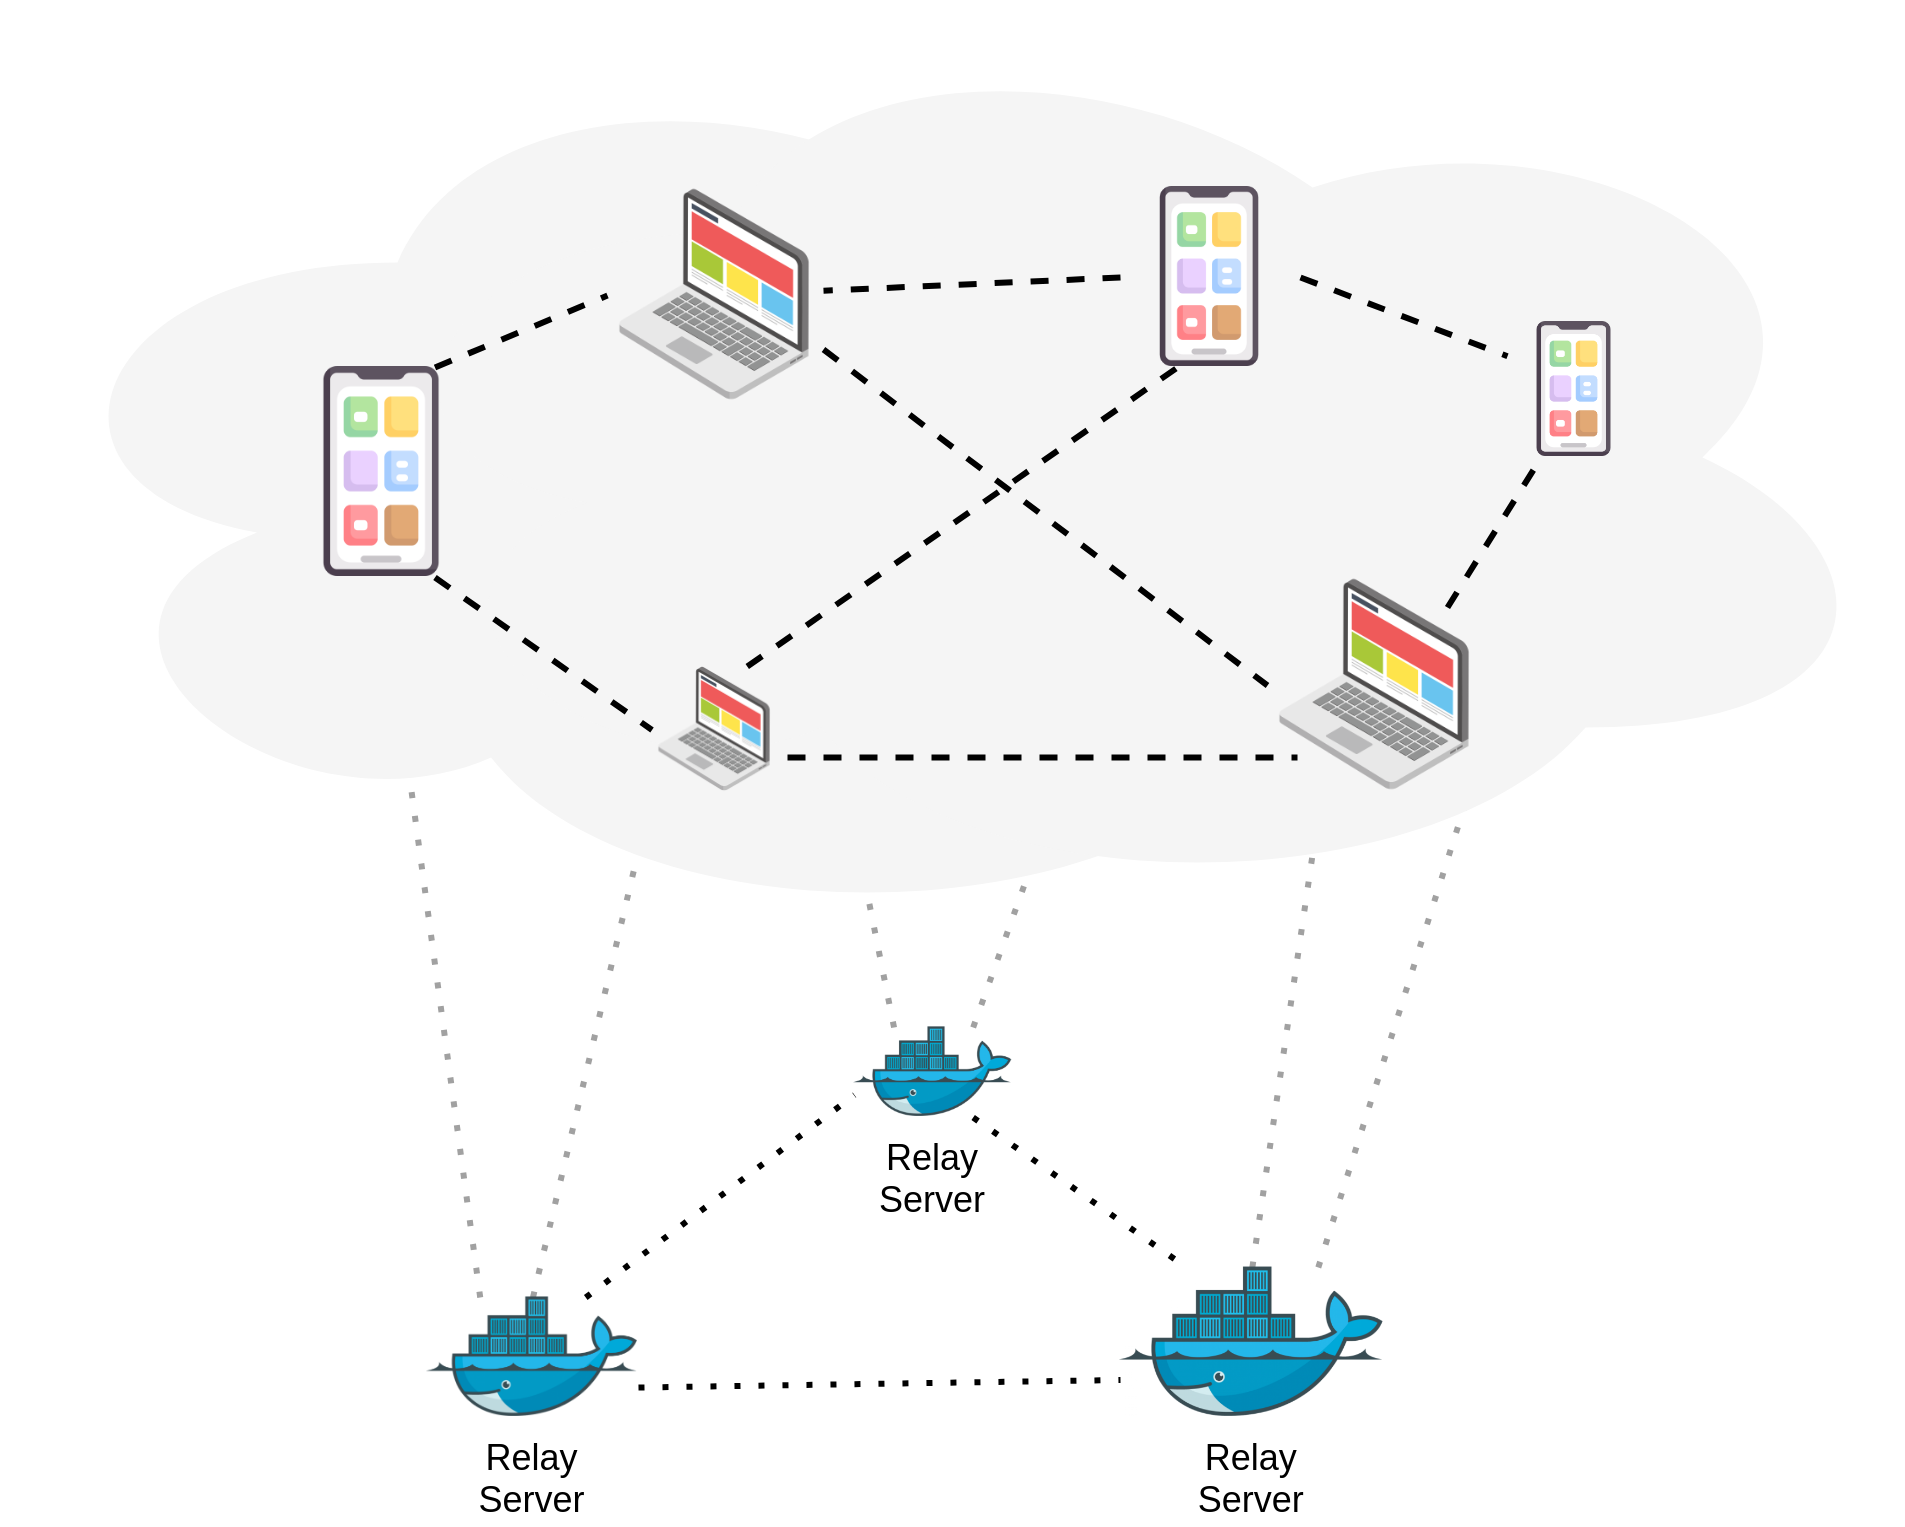
\includegraphics[width=\columnwidth]{in-browser-pow-topology}
  \caption{The topology of the system, with an underlay network of relay servers that allow the overlay network of devices to discover their peers and establish direct connections.}
  \label{fig:in-browser-pow-topology}
\end{figure}

\subsection{Remarks}

The prototype was tested, is demonstrable and works as intended. Some \emph{Nakamoto} chain-based
features were simplified, for the sake of maintaining a didactic complexity. For example, 
the Longest-Chain rule, in this prototype, works by having a temporary set of active blocks 
that get appended to the main chain if there are new blocks mined on top
of them. This setting enforces higher synchrony between the peers, as there is also no mechanism for
general chain data synchronization. Additionally, this means that a new peer joining the network does not
need or does not ask for the rest of the chain history to start mining, but just the most recent block.
The difficulty was also set to a constant value, for the sake of simplicity.
Again, this is justified by the purpose of this prototype, which was to demonstrate the achievement
of consensus in a permissionless environment.

No extensive benchmarks or analysis were made, other than live tests with multiple
and heterogeneous devices. The basic tests involved one, two or more browser tabs
opened in the same device, competing for mining the blocks. The distribution of blocks mined
in a fixed and considerable interval was observed to be uniform for the participants. Another test was
conducted with a laptop and a mobile device, for which, for obvious reasons, the laptop
had a generally bigger advantage in the mining process.

\subsection{Future Work}

The prototype was developed as a proof-of-concept and a demonstration of the feasibility
of the \emph{PoW} consensus protocol in a permissionless environment. The next steps
for this project would be to extend the functionality and the features of the system,
in order to make it more robust and usable. Some ideas for future work are, for example,
the improvement of the \emph{PoW} algorithm, by adding a difficulty adjustment mechanism,
to make the mining process more fair for computationally weaker devices, or to
add a mechanism for the synchronization of the old chain history. Another idea would be to
improve the parallelization of the computations, by more efficiently distributing the
workload among mining threads. Finally, the user interface could be improved 
with more informative and interactive features, that would allow the user to have a 
deeper understanding of the system and the consensus process (See Fig. \ref{fig:in-browser-pow}).

\begin{figure}[h]
  \centering
  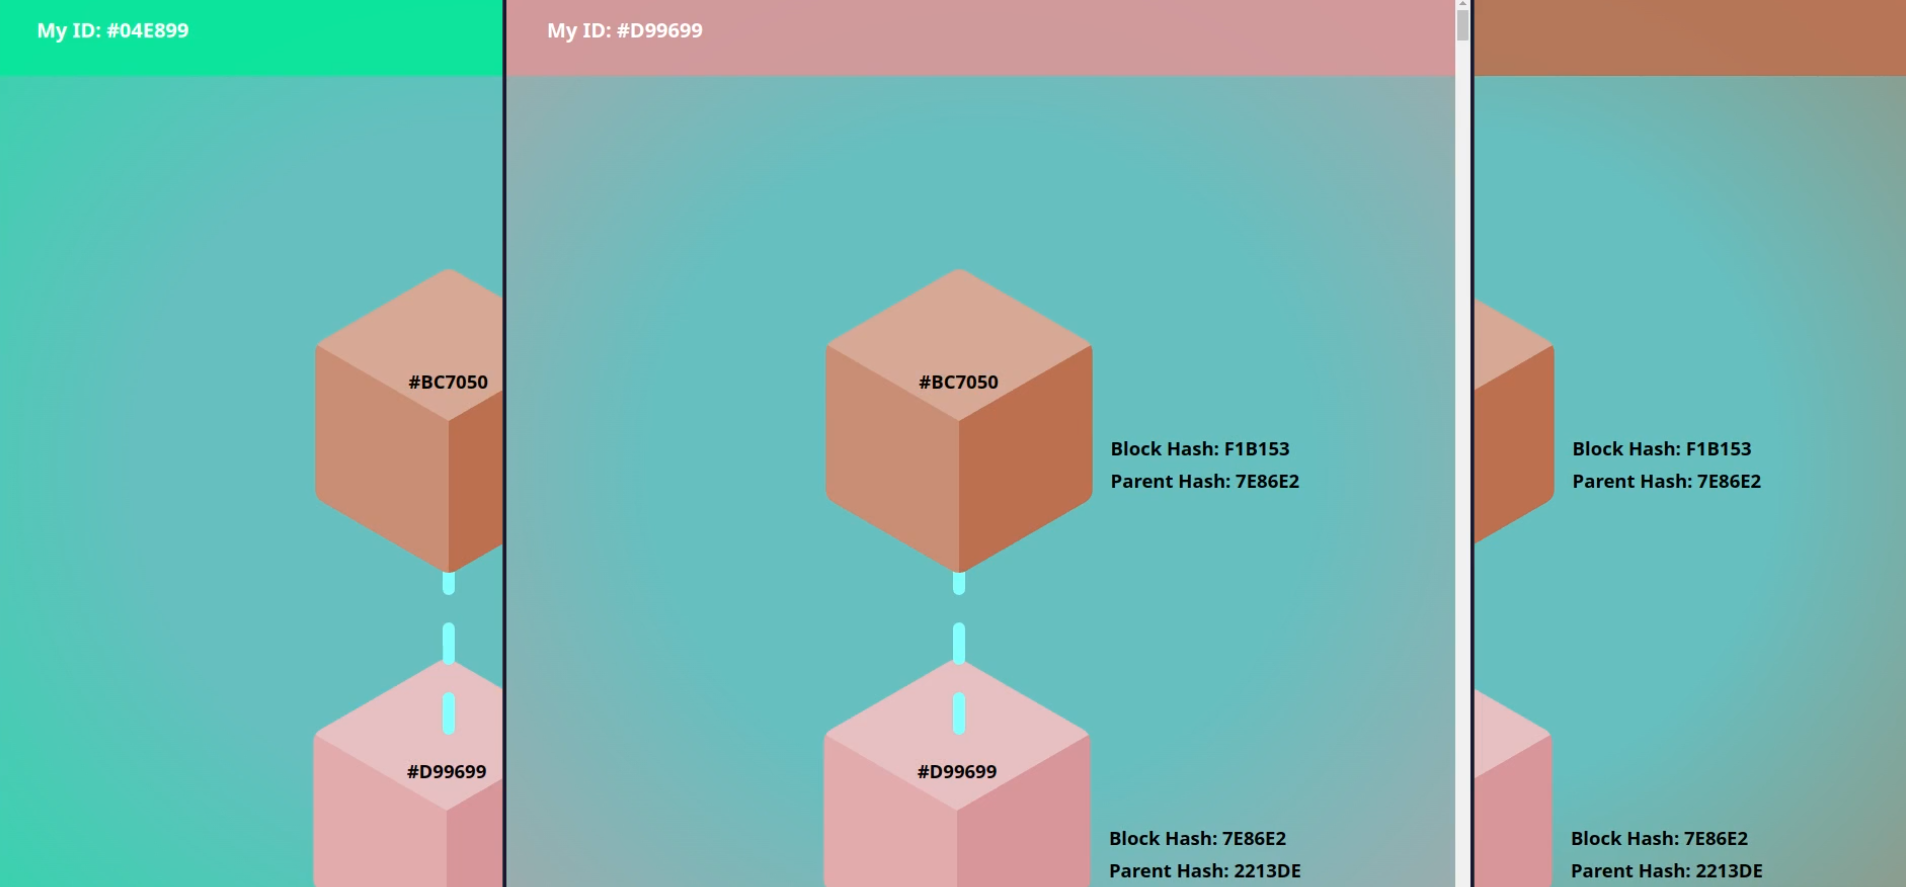
\includegraphics[width=\columnwidth]{in-browser-pow}
  \caption{The user interface showing three browser tabs opened and competing for mining the next blocks, 
  while achieving consensus and presenting the same view.}
  \label{fig:in-browser-pow}
\end{figure}

\subsection{Repository}

All the work developed, both the practical and the theoretical components, can be found 
at \emph{\url{https://github.com/edurbrito/dist-sys-seminar}}.

% that's all folks
\end{document}
